\documentclass[prd,preprintnumbers,onecolumn,eqsecnum,floatfix,letter]{revtex4}
\usepackage{color}
\usepackage{calc}
\usepackage{amsmath,amssymb,graphicx}
\usepackage{amssymb,amsmath}
\usepackage{tensor}
\usepackage{bm}
\usepackage{times}
\usepackage[varg]{txfonts}
\usepackage{mathrsfs,amsmath}  
\usepackage{empheq}
\usepackage[colorlinks, pdfborder={0 0 0}]{hyperref}
\definecolor{LinkColor}{rgb}{0.75, 0, 0}
\definecolor{CiteColor}{rgb}{0, 0.5, 0.5}
\definecolor{UrlColor}{rgb}{0, 0, 0.75}
\hypersetup{linkcolor=LinkColor}
\hypersetup{citecolor=CiteColor}
\hypersetup{urlcolor=UrlColor}
\maxdeadcycles=1000
\allowdisplaybreaks
\textwidth 7.5 in 
\hoffset -1 cm 
\newcommand{\boxedeq}[2]{\begin{empheq}[box={\fboxsep=6pt\fbox}]{align}\label{#1}#2\end{empheq}}
\newcommand{\comment}[1]{\textcolor{blue}{\textit{#1}}}
\newcommand{\Sean}[1]{\textcolor{red}{\textit{Sean:#1}}}
\newcommand{\ashok}[1]{\textcolor{cyan}{\textit{Ashok:#1}}}


\begin{document}

\newcommand{\be}{\begin{equation}}
\newcommand{\ee}{\end{equation}}
\newcommand{\ber}{\begin{eqnarray}}
\newcommand{\eer}{\end{eqnarray}}
\def\bea{\begin{eqnarray}}
\def\eea{\end{eqnarray}}
\newcommand{\etal}{\emph{et al.}}


\title{Notes on applying super momentum balance law to constraint GW waveform \\ (Update on Daily Progress) }
\author{Ashok Choudhary}\email{aschoudhary@mix.wvu.edu}
\author{Sean T. McWilliams}\email{sean.mcwilliams@mail.wvu.edu}
\affiliation{Department of Physics and Astronomy, West Virginia University, Morgantown, WV 26506, USA}

\begin{abstract}
\end{abstract}

\maketitle

\section{Local super momentum balance law}

The local super-momentum balance law for asymptotically flat space-time is given by 
\begin{equation}
\mathcal{F}(\theta,\phi) \Big|^{u_{2}}_{u_{1}}  := -\int_{u_{1}}^{u_{2}} du \left[|\dot{\sigma^{o}}|^{2} - \Re\left(\eth^{2}\dot{\bar{\sigma}}^{o} \right) \right](u, \theta, \phi) = \Re\left[\Psi^{o}_{2} + \bar{\sigma}^{o}\dot{\sigma^{o}}\right]\left(u_{1}, \theta, \phi\right) - \Re\left[\Psi^{o}_{2} + \bar{\sigma}^{o}\dot{\sigma^{o}}\right]\left(u_{2}, \theta, \phi\right) 
\end{equation}
where
\begin{align}
	2 \Re\, \Psi^{o}_{2}\left(u, \theta, \phi \right) & = \lim_{r \to +\infty} r^{3} \, C_{abcd}n^{a}l^{b}n^{c}l^{d}\label{psi2}\\  \Psi^{o}_{4}\left(u, \theta, \phi \right) & = \lim_{r \to +\infty} r \, C_{abcd}n^{a}\bar{m}^{b}n^{c} \bar{m}^{d} = \ddot{\bar{\sigma}}^{o} = r\left(\ddot{h}_{+} + i\, \ddot{h}_{\times}  \right)
	\label{psi4}
\end{align}
We simplify the above equation for the case for perturbed black hole using the results in [add ref]. Equation 2.59 in ref[add ref] the mass aspect
\begin{equation}
	\Psi = \psi^{0}_{2} + \eth^{2}\bar{\sigma}^{o} + {\sigma}^{o}\dot{\bar{\sigma}}^{o}
\end{equation}
and the spherical harmonic expansion of the above result is

\begin{equation}
	\Psi = \Psi^{0} + \Psi^{i}Y^{0}_{1\,i} + + \Psi^{i\,j}Y^{0}_{2\,i\,j}
\end{equation} 

The interior mass and three-momentum with the $l=0$ and $l=1$ harmonic contributions is given by
\begin{align}
	M_{B} = \frac{-c^{2}}{2\sqrt{2}\,G}\Psi^{0}\\
	P^{i} = -\frac{c^3}{6\,G}\Psi^i
\end{align}

Using the above results, at leading order we can relate mass and energy momentum of interior space time to $\psi_2$ as
\begin{equation}
	-2\,\sqrt{2}\,M_B = \Re\left[\psi^{0}_{2} + \eth^{2}\bar{\sigma}^{o} + {\sigma}^{o}\dot{\bar{\sigma}}^{o} \right]
\end{equation}
We can use the above result in the local balance law, to rewrite the local balance law. As a first step just considering change in mass we have
\begin{align}
	 -\int_{u_{1}}^{u_{2}} du \left[|\dot{\sigma^{o}}|^{2} - \Re\left(\eth^{2}\dot{\bar{\sigma}}^{o} \right) \right](u, \theta, \phi) =& -\left[\left(2\sqrt{2}M_B + \eth^{2}\bar{\sigma}^{o}\right)(u_1, \theta, \phi) - \left(2\sqrt{2}M_B + \eth^{2}\bar{\sigma}^{o}\right)(u_2, \theta, \phi)\right]\\ = & \int_{-\infty}^{t} du\, \left(2\sqrt{2}\,\dot{M}_B+ \eth^{2}\bar{\sigma}^{o} \right)\\ \implies -|\dot{\sigma^{o}}|^{2} + \Re\left( \eth^{2}\bar{\sigma}^{o}\right) = 2\sqrt{2}\,\dot{M}_B + \eth^{2}\bar{\sigma}^{o} \\ \implies  -|\dot{\sigma^{o}}|^{2}  = 2\sqrt{2}\,\dot{M}_B  
\end{align}
Higher order corrections can be obtained in a similar way
\section{ Weyl scalar $\Psi^{o}_{2}$ for BOB as perturber cross the light ring }
In Backwards One-Body (BOB)[add ref] description of black hole binary merger, the system is described as a single black hole spacetime with a inspiraling in perturber. At the leading order we can just assume that the mass of the perturber and the source is evolving. 
\begin{figure}
	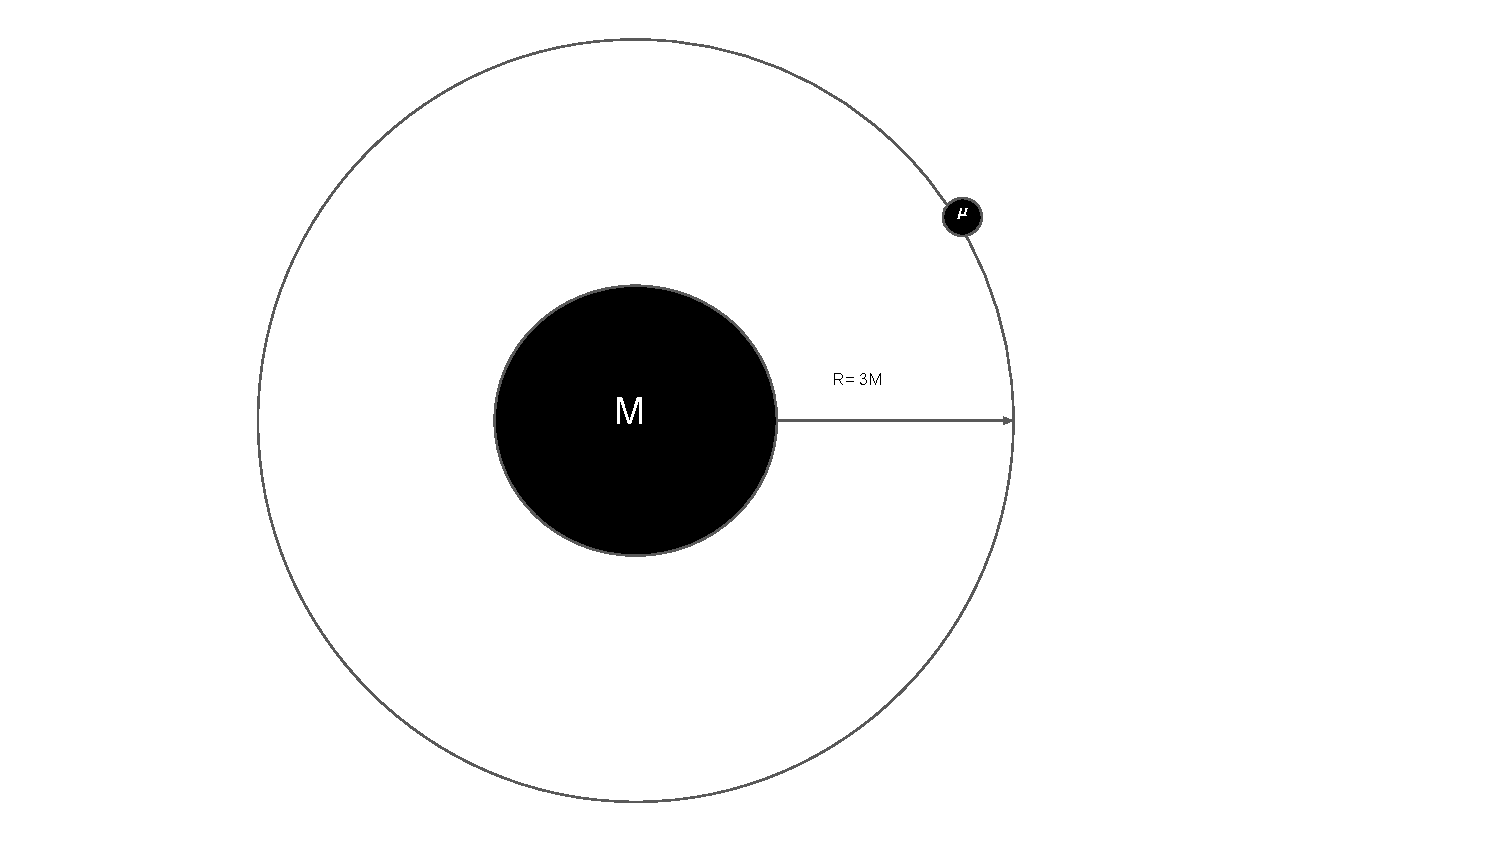
\includegraphics[width=5.5in]{../plots/BOB.pdf}
	\caption{The figure}
	\label{fig:resedualGrowthLogLog}
\end{figure} 
\subsection{Evolution of $\Psi^{o}_{2}$ for perturbed Swarzchild black hole }
We assume that the perturber is loosing mass at given rate $\dot{\epsilon}$. Given this and looking at Bianchi identity on asymptotically flat space time, we can also deduce that the source mass is evolving as $\dot{\epsilon}^2$. In this model where we assume both perturber and source mass evolving in time, we can relate this to gravitational wave strain. The gravitational wave luminosity is given by,
\begin{align}
	\mathcal{L} &= -\frac{dE}{dt} = \lim_{r \to +\infty} \frac{r^2}{16\,\pi}\sum_{l=2}^{\infty}\sum_{m=-l}^{l}\Big|\int_{-\infty}^{\infty}dt'\Psi_{4}^{l\,m}\Big|^2 \nonumber \\
	\text{for l=2, m=2 mode}\\
	\mathcal{L} &=  \lim_{r \to +\infty} \frac{r^2}{16\,\pi}\Big|\int_{-\infty}^{\infty}dt'\Psi_{4}^{2\,m}\Big|^2 \\
	\text{And the News function in related to $\Psi_4$ by} \nonumber\\
\sigma = \int_{-\infty}^{t}dt'\Psi_{4}^{2\,2} 
\end{align}
 Now let us look at how this luminosity evolves with time.
 \begin{align}
 	\frac{d\mathcal{L}_{GW}}{dt} &=  \frac{1}{16\,\pi}\frac{d}{dt}\Big|\int_{-\infty}^{\infty}dt'\Psi_{4}^{2\,2}\Big|^2 = \frac{1}{16\,\pi}\frac{d}{dt}\Big[\int_{-\infty}^{t}dt'\bar{\Psi}_{4}^{2\,2}(t')\int_{-\infty}^{t}dt''\Psi_{4}^{2\,2}(t'')\Big]\\
 	&=\frac{1}{16\,\pi}\Big[\bar{\Psi}_{4}^{2\,2}(t)\int_{-\infty}^{t}dt'\Psi_{4}^{2\,2}(t') + \Psi_{4}^{2\,2}(t)\int_{-\infty}^{t}dt'\bar{\Psi}_{4}^{2\,2}(t')\Big] \nonumber\\
 	&=\frac{1}{16\pi}\Big[\ddot{\bar{\sigma}}(t)\dot{\sigma}(t) + \dot{\bar{\sigma}}(t)\ddot{\sigma}(t)\Big] = \frac{1}{8\pi}\Re\Big[\ddot{\bar{\sigma}}(t)\dot{\sigma}(t)\Big]\nonumber
 \end{align}
 
 \subsubsection{Luminosity from a binary system}
 
 Now let us look at how at leading the luminosity of binary source which is shedding mass evolve with time 
 \begin{align}
 	\mathcal{L}_{GW} & = \frac{32}{5}\frac{M^3\,\mu^2}{r^5}\nonumber\\
 	\frac{d\mathcal{L}_{GW}}{dt} & = \frac{32M^3\mu^2}{5r^5}\Big[\frac{3}{M}\frac{dM}{dt} + \frac{2}{\mu}\frac{d\mu}{dt} - \frac{5}{r}\frac{dr}{dt}\Big]
 \end{align}
 
The radiation reaction has a negligible effect on dynamics of the perturber inside ISCO, so we model the rate of mass loss as source of rate of Luminosity change. The Mass of the central black holes is much larger then the mass of the perturber so in the above equation  

\subsubsection{Mass, Momentum and Angular momentum loss of a perturbed spacetime}
We can use the time evolution of mass aspect, equation 2.58 in ref[add] to relate the news amplitude to the mass and angular momentum loss. 
\begin{equation}
	\dot{\Psi} = \dot{\sigma}\dot{\bar{\sigma}} + k\phi^{0}_{2}\bar{\phi}^{0}_{2}
\end{equation}

In the absence of electromagnetic fields we set the second term in right hand side to zero. The above equation then is related to mass and angular momentum loss of the perturbed space time with the radiated GWs strain. 
\begin{equation}
	\dot{\Psi} = -\frac{2\sqrt{2}G}{c^2}\dot{M} -\frac{6G}{c^3}\dot{P}^iY^{0}_{1\,i} + ...
\end{equation}  

We can use the above results to get an insight into how mass and angular momentum are related. For the case of gravitational wave emitted the merger the waveform is well described by BOB model. We have 
\begin{equation}
	|\psi_4| = A_{p}\text{sech}[\gamma(t-t_p)]
\end{equation}
Since $|\sigma|\approx |\psi|/\omega$ for quasi circular systems. Where $\omega$ is given by
\begin{equation}
	\Omega = \Biggl\{\Omega^{4}_{0} + k\Big[\tanh\Big(\frac{t-t_p}{\tau}\Big) -\tanh\Big(\frac{t_0-t_p}{\tau}\Big)\Big]\Biggr\}^{1/4}
\end{equation}
where the constant k is given by
\begin{equation}
	k = \Bigg[\frac{\Omega^{4}_{QNM} - \Omega^4_{0}}{1-\tanh[(t_0-t_p)/\tau]}\Bigg]
\end{equation}

Using equation 2.6 and 2.7 at leading order, we can relate the mass loss rate to the time derivative of GWs strain. Setting $c = G = 1$ we see that equation 

\begin{equation}
	|\dot{\sigma}|^2 = -2\sqrt{2}\dot{M} = \frac{|\psi_4|^2}{4\Omega^2}
\end{equation}
To look at how the Mass evolves near the peak, we Taylor expand $|\dot{\sigma}|^2$ around the peak.

\end{document}
